% !TeX program = pdflatex
\documentclass[11pt,a4paper]{amsart}

\newcommand{\notelanguage}{finnish}
% Shared preamble for course notes and exercise sets.

\usepackage[T1]{fontenc}
\usepackage{lmodern}
\providecommand{\notelanguage}{english}
\usepackage[finnish,english]{babel}
\AtBeginDocument{\expandafter\selectlanguage\expandafter{\notelanguage}}

\newcommand{\notesfinnishlanguage}{finnish}
\ifx\notelanguage\notesfinnishlanguage
\newcommand{\notestheoremname}{Lause}
\newcommand{\noteslemmaname}{Lemma}
\newcommand{\notespropositionname}{Propositio}
\newcommand{\notescorollaryname}{Seurauslause}
\newcommand{\notesdefinitionname}{Määritelmä}
\newcommand{\notesexamplename}{Esimerkki}
\newcommand{\notesproblemname}{Tehtävä}
\newcommand{\notesexercisename}{Tehtävä}
\newcommand{\notesremarkname}{Huomautus}
\newcommand{\notessolutionname}{Ratkaisu}
\else
\newcommand{\notestheoremname}{Theorem}
\newcommand{\noteslemmaname}{Lemma}
\newcommand{\notespropositionname}{Proposition}
\newcommand{\notescorollaryname}{Corollary}
\newcommand{\notesdefinitionname}{Definition}
\newcommand{\notesexamplename}{Example}
\newcommand{\notesproblemname}{Problem}
\newcommand{\notesexercisename}{Exercise}
\newcommand{\notesremarkname}{Remark}
\newcommand{\notessolutionname}{Solution}
\fi

\usepackage[a4paper,margin=30mm]{geometry}
\usepackage{microtype}
\usepackage{graphicx}
\usepackage{enumitem}

\newcommand{\exerciseheading}[2]{%
  \par\noindent
  {\large\bfseries #1\par}
  \vspace{0.1em}
  \noindent{\large #2\par}
  \vspace{1.5em}
}

\usepackage{amsmath}
\usepackage{amssymb}
\usepackage{amsthm}
\usepackage{mathtools}
\usepackage{aliascnt}

% Linear systems: the argument gives the number of alignment pairs.
\newenvironment{linearsystem}[1]
  {\left\{\begin{alignedat}{#1}}
  {\end{alignedat}\right.}

\usepackage[hidelinks,pdfusetitle]{hyperref}

\numberwithin{equation}{section}
\setlist{itemsep=0.25em,topsep=0.5em}

\theoremstyle{plain}
\newtheorem{theorem}{\notestheoremname}[section]
\newaliascnt{lemma}{theorem}
\newtheorem{lemma}[lemma]{\noteslemmaname}
\aliascntresetthe{lemma}
\newaliascnt{proposition}{theorem}
\newtheorem{proposition}[proposition]{\notespropositionname}
\aliascntresetthe{proposition}
\newaliascnt{corollary}{theorem}
\newtheorem{corollary}[corollary]{\notescorollaryname}
\aliascntresetthe{corollary}

\theoremstyle{definition}
\newaliascnt{definition}{theorem}
\newtheorem{definition}[definition]{\notesdefinitionname}
\aliascntresetthe{definition}
\newaliascnt{example}{theorem}
\newtheorem{example}[example]{\notesexamplename}
\aliascntresetthe{example}
\newaliascnt{problem}{theorem}
\newtheorem{problem}[problem]{\notesproblemname}
\aliascntresetthe{problem}
\newtheorem{exercise}{\notesexercisename}

\theoremstyle{remark}
\newaliascnt{remark}{theorem}
\newtheorem{remark}[remark]{\notesremarkname}
\aliascntresetthe{remark}

\newenvironment{solution}
{
\begin{proof}[\notessolutionname]}
  {
\end{proof}}

\usepackage[nameinlink,noabbrev]{cleveref}

\crefname{theorem}{theorem}{theorems}
\crefname{lemma}{lemma}{lemmas}
\crefname{proposition}{proposition}{propositions}
\crefname{corollary}{corollary}{corollaries}
\crefname{definition}{definition}{definitions}
\crefname{example}{example}{examples}
\crefname{problem}{problem}{problems}
\crefname{exercise}{exercise}{exercises}
\crefname{remark}{remark}{remarks}

\ifx\notelanguage\notesfinnishlanguage
\crefname{theorem}{lause}{lauseet}
\crefname{lemma}{lemma}{lemmat}
\crefname{proposition}{propositio}{propositiot}
\crefname{corollary}{seurauslause}{seurauslauseet}
\crefname{definition}{määritelmä}{määritelmät}
\crefname{example}{esimerkki}{esimerkit}
\crefname{problem}{tehtävä}{tehtävät}
\crefname{exercise}{tehtävä}{tehtävät}
\crefname{remark}{huomautus}{huomautukset}
\fi

\newcommand{\NN}{\mathbb{N}}
\newcommand{\NNone}{\mathbb{N}_1}
\newcommand{\ZZ}{\mathbb{Z}}
\newcommand{\QQ}{\mathbb{Q}}
\newcommand{\RR}{\mathbb{R}}
\newcommand{\CC}{\mathbb{C}}
\newcommand{\PP}{\mathbb{P}}

\DeclareMathOperator{\im}{im}
\DeclareMathOperator{\rank}{rank}
\DeclareMathOperator{\syt}{syt}
\DeclarePairedDelimiter{\abs}{\lvert}{\rvert}
\DeclarePairedDelimiter{\norm}{\lVert}{\rVert}
\newcommand{\set}[1]{\left\lbrace#1\right\rbrace}
\newcommand{\maxset}[1]{\max\set{#1}}
\newcommand{\minset}[1]{\min\set{#1}}
\newcommand{\powerset}[1]{\mathcal{P}\!\left(#1\right)}


\title{Johdatus logiikkaan II\\Harjoituksen 1 ratkaisut}
\author{}
\date{}

\begin{document}

\exerciseheading{Johdatus logiikkaan II}{Harjoituksen 1 ratkaisut}

\begin{exercise}
  Mikä aakkosto kuuluu mihinkin malliin? Mikä on jäljelle jäävän
  mallin aakkosto?
  \[
    L_1 = \{P_1, P_2, c_0\},\qquad
    L_2 = \{P_3, P_8\},\qquad
    L_3 = \{R_0, c_0\}.
  \]
  \begin{center}
    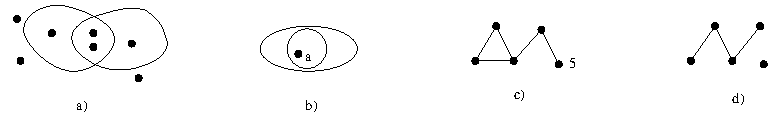
\includegraphics[width=\linewidth]{figures/exercise-01-models.pdf}
  \end{center}
\end{exercise}

\begin{exercise}
  Anna esimerkki \(L\)-mallista, kun
  \begin{enumerate}[label=(\alph*)]
    \item \(L = \{R\}\),
    \item \(L = \{P, R\}\),
    \item \(L = \{R_0, R_1, c_0\}\),
    \item \(L = \{P, c\}\),
    \item \(L = \varnothing\).
  \end{enumerate}
  Tässä \(P\) on aina yksipaikkainen ja \(R\) tai \(R_i\) kaksipaikkainen
  relaatiosymboli.
\end{exercise}

\begin{exercise}
  Olkoon \(\mathcal M\) seuraava malli:
  \begin{center}
    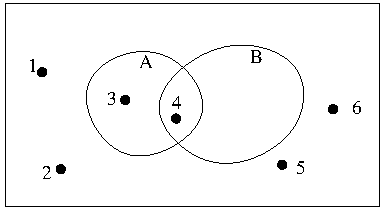
\includegraphics[width=0.5\linewidth]{figures/exercise-01-model.pdf}
  \end{center}
  \begin{enumerate}[label=(\alph*)]
    \item Minkä aakkoston malli \(\mathcal M\) on?
    \item Mikä on \(\operatorname{dom}(\mathcal M)\)?
    \item Mitkä ovat aakkoston symbolien tulkinnat?
  \end{enumerate}
  Ovatko vastaukset yksikäsitteiset?
\end{exercise}

\begin{exercise}
  Anna aakkoston \(\{P_0, P_1, P_2\}\) malli, jossa predikaatit jakavat mallin
  universumin kuuteen erilliseen, epätyhjään osaan (\(P_i\) ovat yksipaikkaisia
  predikaattisymboleita).
\end{exercise}

\begin{exercise}
  Olkoon \(L = \{P_0, c_0\}\). Anna esimerkki \(L\)-malleista \(\mathcal M\)
  ja \(\mathcal M'\), s.e. kaikki seuraavat pätevät:
  \begin{itemize}
    \item \(\operatorname{dom}(\mathcal M) \ne
      \operatorname{dom}(\mathcal M')\),
    \item \(P_0^{\mathcal M} = P_0^{\mathcal M'}\),
    \item \(c_0^{\mathcal M} \in P_0^{\mathcal M}\), mutta
      \(c_0^{\mathcal M'} \notin P_0^{\mathcal M'}\).
  \end{itemize}
\end{exercise}

\begin{exercise}
  Tarkastellaan muotoa
  \[
    \mathcal M = (X, \{(0,1), (1,1), (2,0)\}, (0,1))
  \]
  olevaa mallia. Anna esimerkki joukosta \(X\) ja aakkostosta \(L\), joilla
  \(\mathcal M\) on \(L\)-malli.
\end{exercise}

\begin{exercise}
  Mitkä seuraavista ovat predikaattilogiikan termejä/kaavoja/ei kumpaakaan
  (kun sallitaan materiaalissa mainittuja lyhennysmerkintöjä
  \(x, y, z, \ldots\) muuttujille, ja \(P, P_i, R, R_i\) relaatioille)?
  Termien ja kaavojen kohdalla kerro myös, mitä symboleita
  aakkostossa on oltava?
  \begin{enumerate}[label=(\alph*)]
    \item \(c_7\)
    \item \(z\)
    \item \(x = y\)
    \item \(\forall y\, P(x)\)
    \item \(\forall x\, x = y\)
    \item \(\forall x\, x\)
    \item \(\neg x_1 = x_1\)
    \item \((x \land z)\)
    \item \((P(x) \land R(x,x))\)
    \item \((\forall x\, x = y \land R(y,z))\)
    \item \(P_0\)
    \item \(\forall x\exists x R(x,x)\)
    \item \((\forall x \land \exists y R(x,y))\)
    \item \(\exists x R(x,\exists y)\)
  \end{enumerate}
\end{exercise}

\begin{exercise}
  (Pohjustusta semantiikkaan) Miten kirjoittaisit luonnolliselle kielelle kaavat
  \begin{enumerate}[label=(\alph*)]
    \item \(\forall x P(x)\), kun tarkasteltavana mallina on ämpäreiden joukko,
      ja \(P\) merkitsee ominaisuutta 'olla sininen'.
    \item \(\forall x\exists y R(x,y)\), kun tarkasteltavana mallina on
      luonnollisten lukujen joukko, ja \(R\) merkitsee järjestystä \(<\).
    \item \(\exists x(R(x,y) \land P(x))\), kun tarkasteltavana joukkona on
      osaston opettajien joukko, \(R\) merkitsee relaatiota 'olla pidempi kuin'
      ja \(P\) ominaisuutta 'käyttää silmälaseja'.
  \end{enumerate}
\end{exercise}

\noindent\textbf{Haastetehtävä.} Toisinaan predikaattilogiikka
esitetään muodossa,
jossa aakkostoissa on vain relaatio- ja funktiosymboleita. Tällöin
sallitaan myös
0-paikkaiset funktiot ja relaatiot. Mitä ne vastaavat?

\end{document}
